% Vstupní vrstva (Data Ingestion): Jaké moduly se starají o komunikaci ven (Git fetcher, GitHub API klient, Team API klient).
% Zpracování a agregace: Kde dochází ke sloučení dat (např. spárování uživatele z Gitu s uživatelem z GitHubu a přiřazení do týmu z Team API).
% Úložná vrstva (Database): Místo, kam se normalizovaná data ukládají.
% Prezentační vrstva: Backendové API (Rust), které vystavuje endpointy pro frontend, a samotná Vue.js aplikace.

\section{Architektura systému}
\label{sec:architecture}
\todo{korektura všeho aaaaaaaa}
tato kapitola popisuje jak byla navržena architektura systému. Bude zde popsáno jaké moduly systém obsahuje a jak spolu moduly komunikují.

Celková architektura systému je znázorněna na \customref{obrázku}{fig:architecture:overall_architecture}.

\begin{figure}[H]
	\centering
	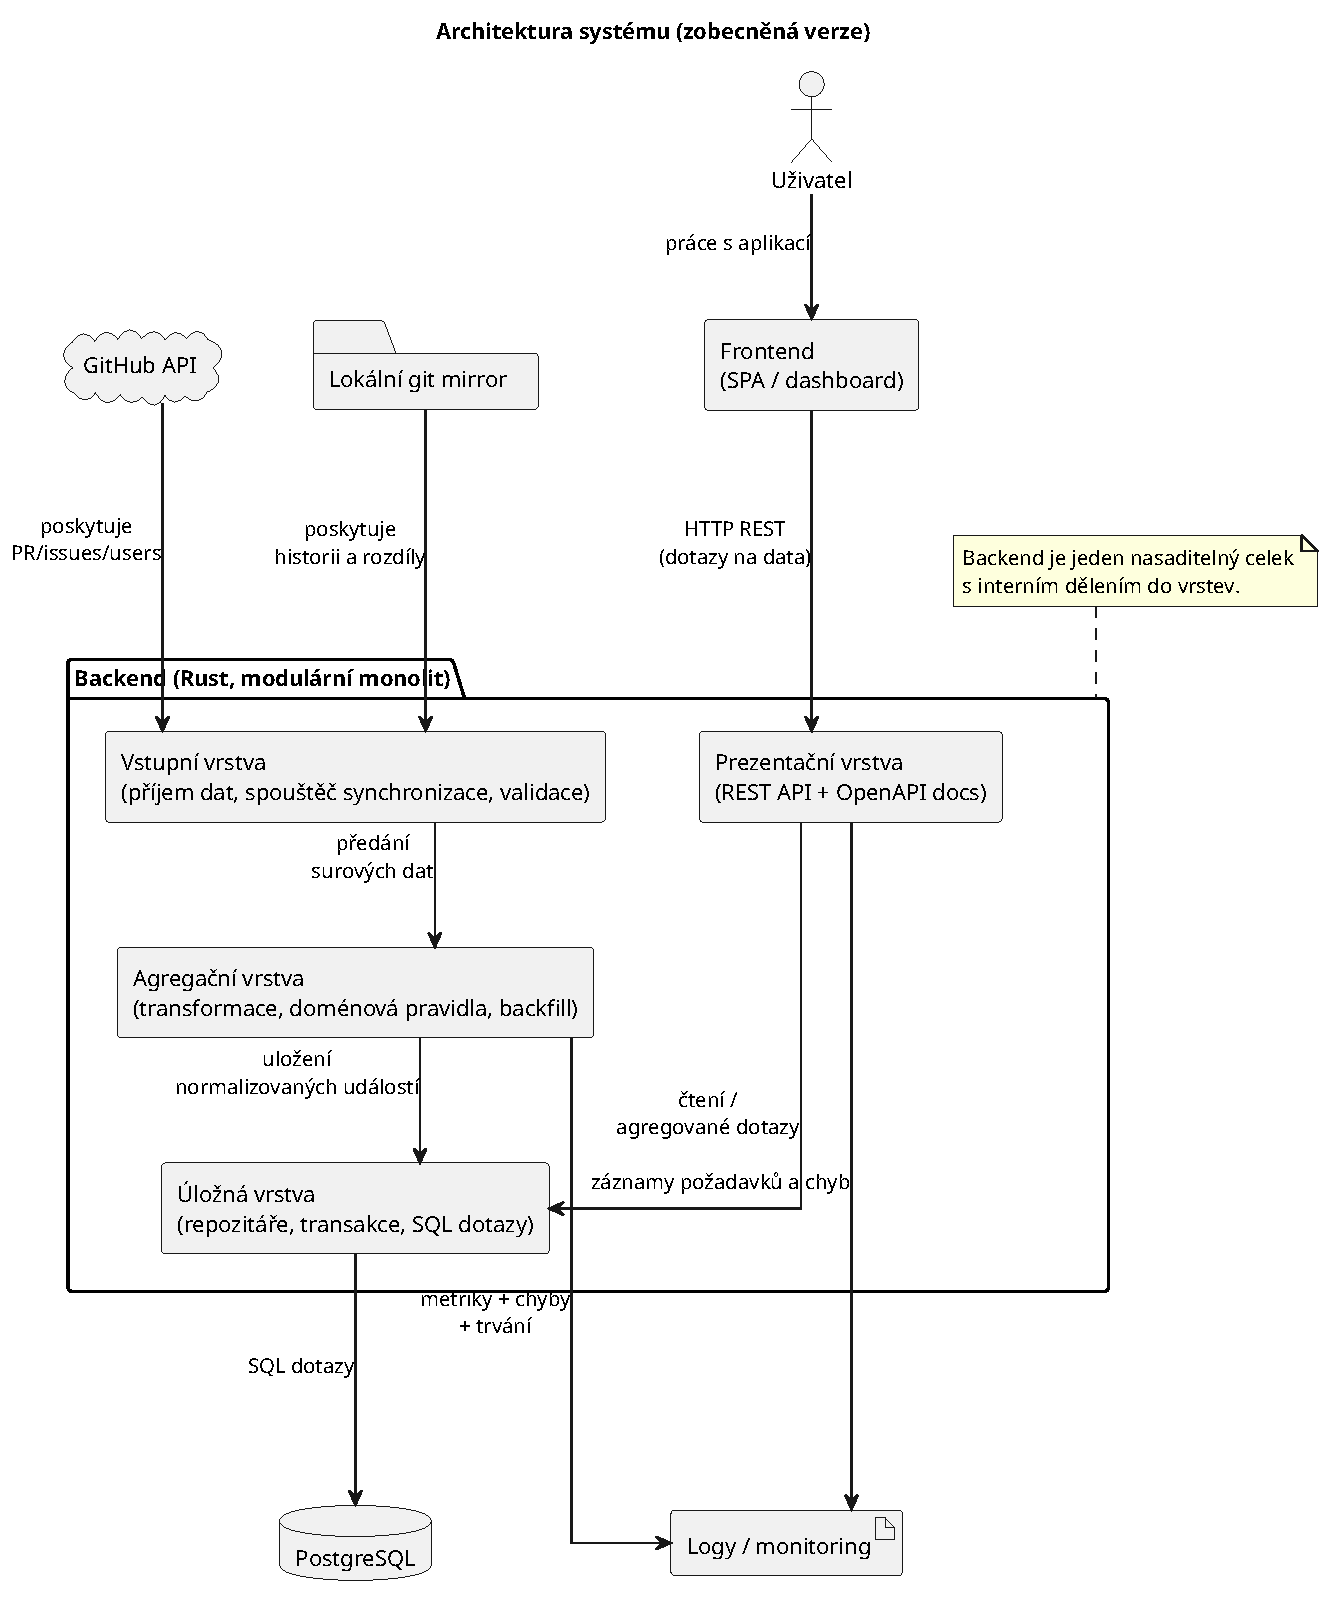
\includegraphics[width=\textwidth]{figures/architecture/overall_architecture.pdf}
	\caption{Celková architektura systému}
	\label{fig:architecture:overall_architecture}
\end{figure}

Systémje navržen jako monolitická aplikace s vrstvenou strukturou (API, aplikační/integrační logika, prezentační vrstva). Vstvená struktura je dosažena za pomocí SoC. Tento přístup umožnuje snoadou rozšířitelnost a vyskokou udržitelnost. Tento monolit poté je v rámci klient serverové architektury rozdělen na backendovou část, která je implementována v Rustu a stará se o zpracování dat a vystavení API pro frontend, a frontendovou část, která je implementována ve Vue.js a stará se o zobrazení dat uživatelům.

\subsection{vstupní vrstva}
Vstupní vrstva se stará o komunikaci s externími zdroji dat. Obsahuje moduly pro komunikaci s GitHub API, Team API a pro načítání dat z git repozitáře.

Stará se o načítání issues a pull requestů z GitHub API, a taktéž se stará o mapování změněných souborů k pull requestům z github repozitáře pokud je daný pr mergnutý.

\subsection{zpracování a agregace}
Tento modul se stará o zpracování transformaci a obecně orchestraci dat získaných z vstupní vrstvy. Zde dochází ke sloučení dat například z GitHub API a Team API, aby bylo možné přiřadit uživatele z Gitu do týmů z Team API.

Tato vrstva vhondě transformuje data pro vložení do databáze a zajištuje že data jsou v konzistentním stavu. taktéž zde probíhá měření trvání jednotlivých operací jako je trvání načtení dat ze vstupní vrstvy a nebo vkládání dat do databáze.

\subsection{úložná vrstva}
Úložná vrstva se stará o ukládání normalizovaných dat do databáze. Tato vrstva poskytuje rozhraní pro ukládání a načítání dat pro zpracování a prezentační vrstvu.

Zde se používají tzv upserty pro zajištění konzistence dat a pro zajištění toho že data jsou v aktuálním stavu. Tato vrstva také zajištuje migrace schématu a evoluci databáze a indexů v průběhu vývoje systému.

\subsection{prezentační vrstva}
Prezentační vrstva se stará o vystavení dat pro uživatele. Obsahuje backendové API které poskytuje endpointy pro frontend a samotnou Vue.js aplikaci, která zobrazuje data uživatelům.

API je navrženo za pomocí REST principů a poskytuje přímé endpointy pro frontend pro získání dat. api je rozděleno do modulů podle usecase nebo dat která se žádají z fe. endpointy jsou zdokumentovány a poskytují i příklady odpovědí a errorů s možností spustit si vlastní request na dané enpointy. Tyto endpointy poté volají primárně databázovou vrstvu pro získání dat. Jedná se o tenkou vrstvu nad databází.

\subsection{průběžné vlastnosti systému}
první vlastností co je přes celý projekt je observabilita a monitorování růběžnohío chování systému. Systém měří délku trvání nejdůležitějších operací což umožnuje identifikovat bottlenecky a taktéž dlouhotrvající procesy jsou opatřeny vizualizací průběhu pokud je to možné průběh vizualizovat v reálném čase. Systém také loguje důležité události a chyby zvlášť pro pozdější analýzu a debugování.

Další vlastností celého systému je robustnost a odolnost vůči chybám a výpadkům. Systém je navržen tak že při chybě ať už z externích api nebo z interní databáze se systém zaloguje chybu a pokusí se pokračovat v běhu. tato vlastnost spolu s možností znovunačítání dat při výpadku zajištuje že systém je stále funkční a poskytuje aktuální data i při dočasných problémech s externími zdroji dat nebo interními chybami.
